%% The first command in your LaTeX source must be the \documentclass command.
%%
%% Options:
%% twocolumn : Two column layout.
%% hf: enable header and footer.
\documentclass[
% twocolumn,
% hf,
]{ceurart}

%%
%% One can fix some overfulls
% \sloppy

%%
%% Minted listings support 
%% Need pygment <http://pygments.org/> <http://pypi.python.org/pypi/Pygments>
\usepackage{minted}
%% auto break lines
\setminted{breaklines=true}

%%
%% end of the preamble, start of the body of the document source.
\begin{document}

%%
%% Rights management information.
%% CC-BY is default license.
\copyrightyear{2021}
\copyrightclause{Copyright for this paper by its authors.
  Use permitted under Creative Commons License Attribution 4.0
  International (CC BY 4.0).}

%%
%% This command is for the conference information
\conference{D2R2’23: Second International Workshop on Linked Data-driven Resilience Research 2023}

%%
%% The "title" command
\title{From Data to Insights: Constructing Spatiotemporal Knowledge Graphs for City Resilience Use Cases}

%%
%% The "author" command and its associated commands are used to define
%% the authors and their affiliations.

\author[1,2]{Amin Anjomshoaa}[%
orcid=0000-0001-6277-742X,
email=Amin.Anjomshoaa@wu.ac.at]

\address[1]{Vienna University of Economics and Business, Welthandelsplatz 1, 1020 Vienna, Austria}
\address[2]{Complexity Science Hub Vienna, Josefstaedter Strasse 39, 1080 Vienna, Austria}
\address[3]{Corvinus University of Budapest, F\H{o}vám tér 8, 1093 Budapest, Hungary}
\address[4]{Centre for Economic and Regional Studies, Tóth Kálmán u. 4, 1097 Budapest, Hungary}

\author[1,2]{Hannah Schuster}[%
orcid=0000-0003-3032-1959,
email=Hannah.Schuster@wu.ac.at]

\author[3,4]{Johannes Wachs}[%
orcid=0000-0002-9044-2018,
email=johannes.wachs@uni-corvinus.hu]

\author[1,2]{Axel Polleres}[%
orcid=0000-0001-5670-1146,
email=Axel.Polleres@wu.ac.at]

%%
%% The abstract is a short summary of the work to be presented in the
%% article.
\begin{abstract}
Data integration plays a crucial role in crisis management and city resilience use cases by enabling the consolidation of information from scattered sources into a unified view, thereby allowing decision-makers to gain a more complete and accurate understanding of the situation at hand. In this paper, we introduce the CRISP Knowledge Graph, constructed from various data resources to present a uniform view of infrastructure networks and services pertinent to crisis management to enable informed and targeted interventions to address crises management use cases. We  provide a brief explanation of the semantic model and its significance in building a comprehensive knowledge graph and then outline our approach for incorporating some large spatiotemporal datasets into this framework, considering the unique challenges that arise in this process.

\end{abstract}

%%
%% Keywords. The author(s) should pick words that accurately describe
%% the work being presented. Separate the keywords with commas.
\begin{keywords}
  Knowledge Graph \sep
  City Resilience \sep
  Crisis Management
\end{keywords}

%%
%% This command processes the author and affiliation and title
%% information and builds the first part of the formatted document.
\maketitle



%%%%%%%%%%%%%%%%%%%%%%%%%%%%%%%%%%%%

\section{Introduction}

During a crisis, data may be scattered across multiple systems, organizations, and agencies, making it difficult to obtain a complete picture of the situation. Furthermore, our built environment is made up of various complex and interrelated systems and services that draw upon various infrastructure networks such as the communication network, the power network, and the transportation network. Understanding the interdependencies of these networks is of great importance for crisis management and can offer insights into dynamics of crises. This in turn allows us to implement informed and targeted interventions that address the root causes and prevent the recurrence of similar crises in the future.

The CRISP Project (Crisis Response and Intervention Supported by Semantic Data Pooling) represents a data-driven approach to Crisis Response and Intervention. It considers both the short-term management of disasters as well as long-term economic impact assessments, at fine-grained regional and temporal granularity. For this purpose, CRISP ingests data from multiple heterogeneous sources and creates a comprehensive and continuously updated data pool, which represents a key asset for semantic modeling and impact forecasting. CRISP aims to increase the transparency of crisis response and intervention processes via a uniform and comprehensive knowledge graph that includes relevant information about infrastructure elements, service networks, and their vulnerability to different types of shock and stress.

In this paper, we present the architecture of CRISP KG as a holistic and efficient medium for bridging the information gap among organizations and crisis management processes. The CRISP KG aims to help allocate resources more effectively and efficiently, identify gaps in services, and assess the long-term impact of the crisis on individuals and communities. By collecting, analyzing, and sharing data in real-time, crisis response and intervention efforts can be better coordinated, more responsive, and more effective, ultimately helping to mitigate the impact of crises and support the recovery of affected communities. To this end, we describe the integration process of various urban networks and spatiotemporal resources to address the specific requirements of crisis management scenarios. Our approach involves connecting urban networks and their corresponding elements to various shock and stress elements, which enables the detection of affected components in a crisis situation. By leveraging this capability, decision-makers can take informed actions to mitigate the impact of crises.

%%%%%%%%%%%%%%%%%%%%%%%%%%%%%%%%%%%%
\section{Semantic Model for Crisis Management}

City resilience refers to a city's ability to adapt and recover from unexpected events or crises, such as natural disasters or pandemics. Knowledge management plays a crucial role in building city resilience by facilitating the sharing and dissemination of relevant information among stakeholders. Effective knowledge management systems can help cities anticipate and respond to emerging threats, identify best practices, and foster innovation. By leveraging the collective knowledge and expertise of its residents, organizations, and government agencies, cities can enhance their resilience and become better equipped to navigate uncertain and challenging times \cite{desouza2013designing,ribeiro2019urban}. Ultimately, city resilience and knowledge management are mutually reinforcing concepts that are essential for building sustainable and thriving communities.

In this context, the CRISP KG aims to establish the backbone of information integration for gathering Austrian infrastructure systems pertinent for crisis management. It offers a comprehensive and collective view of urban infrastructure, service networks, and diverse environmental indicators. By connecting data on population, medical services, weather, transport, and utilities, CRISP KG gives users a way to understand how interconnected systems react to crisis and shock situations. \textbf{CRISP KG is built on the foundation of three core elements: event of hazards, geographical regions, and infrastructure networks}. These three elements are cornerstones of our crisis management framework and its functionality (see Fig. \ref{overview}). 


\begin{figure}
  \label{overview}
  \centering
  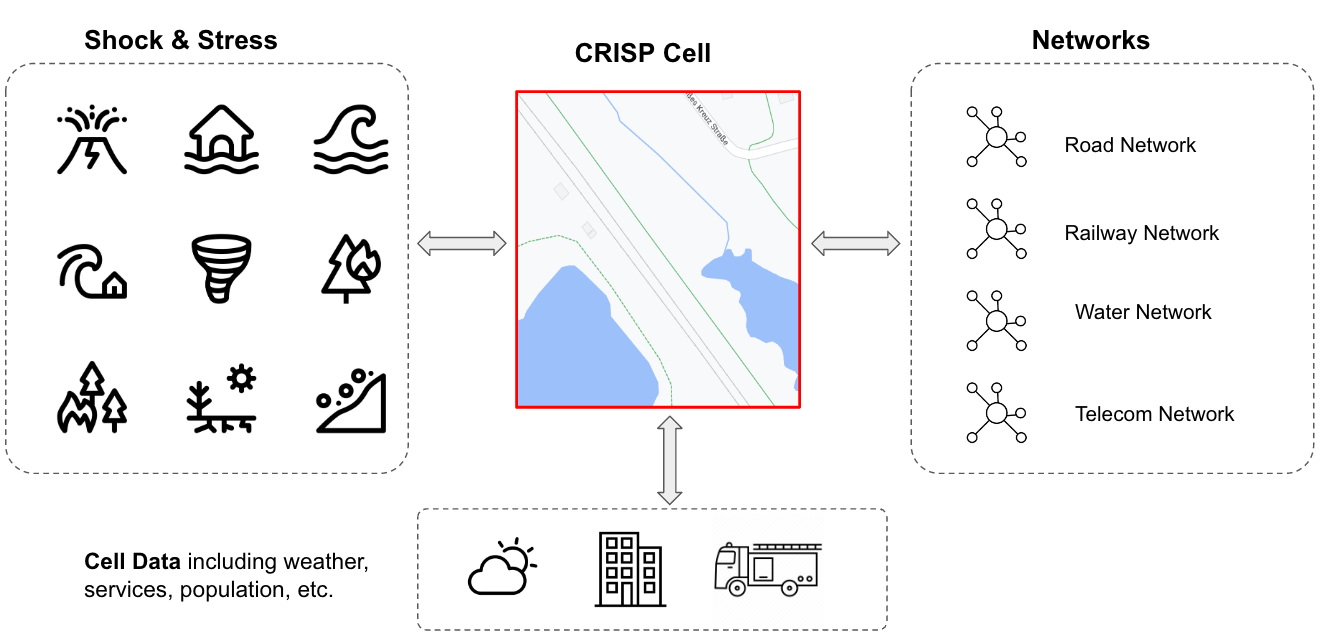
\includegraphics[scale=0.25]{images/Crisp_Overview}
  \caption{Overview of Knowledge Graph Components.}
\end{figure}


Hazards consist of two main components: shocks and stresses. Shocks are sudden, intense events typically associated with large-scale disasters such as earthquakes, hurricanes, or terrorist attacks. On the other hand, stresses are the gradual factors that can weaken a community's resilience. Stresses can be caused by a variety of factors, such as climate change, population growth, urbanization, and economic instability. We use the INSPIRE categories introduced by the European Union spatial data infrastructure (SDI) initiative to classify hazards \cite{bartha2011standardization}. 

Because hazard events can occur without regard for political borders, we utilize a grid cell system to organize both the events and infrastructure. Once organized into grid cells, we then assign the events and infrastructure to overlapping regions, such as communities, cities, and states. By doing so, we can connect the hazard events to infrastructure in a more effective and efficient manner, regardless of where they may occur. This approach allows for a more holistic understanding of hazards and their impacts, ultimately leading to better preparedness and response efforts. The selected grid cells in CRISP are one square kilometer cells defined by the Austrian Central Institute for Meteorology and Geodynamics \cite{haiden2011integrated}. All regions including political regions (e.g. communities, districts, states) and service regions (e.g. hospital and fire-brigade care zones) are defined as spatial features and mapped to underlying grid cells. Depending on specific use cases and their involved regions, infrastructure elements that are assigned to grid cells may be allocated to multiple overlaying regions.


Finally, the infrastructure networks refer to the interconnected relationships and dependencies between different cells, which can be visualized as a complex web of interactions. These networks define the physical elements of interconnected systems that are necessary to support, maintain, or improve the living conditions of society by providing essential goods and services, collectively known as urban infrastructure. In the case of the CRISP KG, this refers to the collection of physical structures assigned to a specific grid cell that delivers essential services. We define two categories: those that are part of a network, like road segments of a street network, and those that operate independently, such as hospitals and fire stations. Many infrastructure elements are themselves dependent on each other. A malfunction in one infrastructure can cause disruptions to the services provided by dependent infrastructure and networks. For example communication or transport network failures can impact the operation of hospitals.



%%%%%%%%%%%%%%%%%%%%%%%%%%%%%%%%%%%%


\section{Big Data Challenge}


Native RDF triple storage and relational-to-RDF translations are two distinct methods of storing and managing RDF data. Native RDF triple stores are optimized for the efficient storage and retrieval of RDF triples and enable querying of the data using SPARQL. However, for large amounts of data, the size of a native RDF triple store can increase significantly, making it less practical for some use cases. Relational-to-RDF translations provide a familiar storage environment and allow RDF data to be stored in traditional relational databases, which are widely used and well-understood by many organizations.

CRISP KG includes concepts and properties describing observations and relevant spatiotemporal data, like weather and climate data, social media, and population data as well as demographics. The weather data provides detailed measurements at a fine-grained level of one measurement per day and per square kilometer, including indicators such as temperature, humidity, radiation, and wind speed. Best practices for semantic sensor networks recommend enriching raw sensor data by including additional information such as the feature of interest, the observed property, the sampling strategy used, and other relevant details \cite{janowicz2019sosa}. Consequently, we would need a dozen of triples for a single spatiotemporal measurement to represent the raw measurement and its context. Austrian weather data in the CRISP KG consists of more than $720$ million measurements per year,  dating back to 2011 \cite{haiden2011integrated}. In order to include this amount of spatiotemporal data in CRISP KG, we follow a Relational-to-RDF approach. We utilize PostgresSQL tables to store large amounts of data and take advantage of built-in features such as table partitions and indexes. This enables us to store the data in a highly scalable way and to query data efficiently. Fig. \ref{crisp_architecture} depicts the overall architecture of the CRISP KG for storage and query of spatiotemporal data.  


\begin{figure}
  \centering
  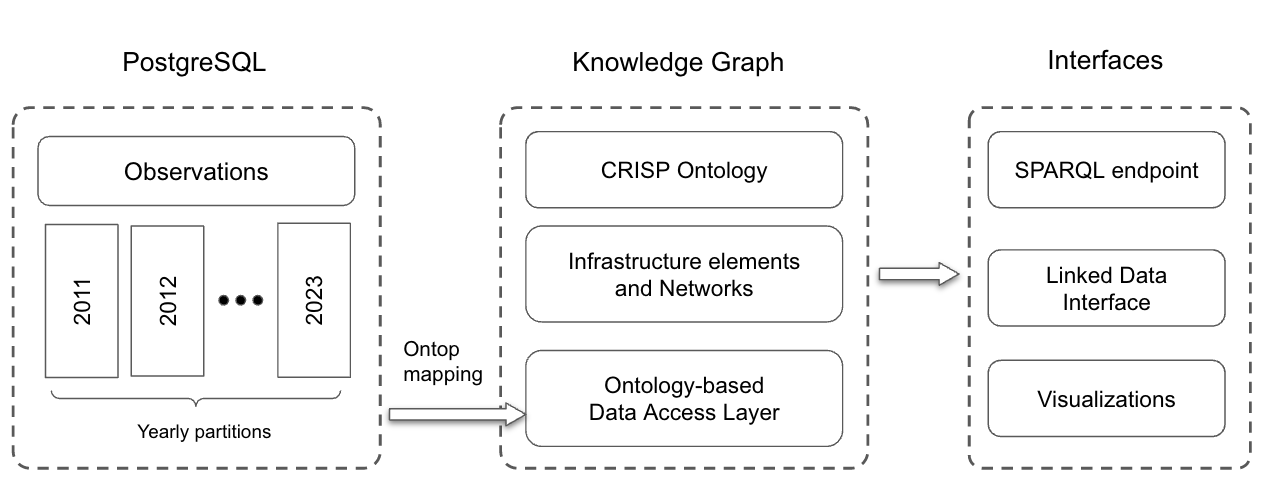
\includegraphics[width=\linewidth]{images/CRISP_architecture.png}
  \caption{Architecture of CRISP project for creating and accessing relevant data for crisis management.}
  \label{crisp_architecture}
\end{figure}


In order to include the RDF representation of the sensor data stored in relational tables, we use the Ontop Virtual Knowledge Graph system \cite{xiao2020virtual} which relies on R2RML mappings and translates SPARQL queries expressed over the knowledge graphs into SQL queries executed by the PostgreSQL database. As an example, Fig. \ref{zamg_mapping} shows the definition of Ontop mapping for weather measurements and their corresponding SQL query (on the left ) and the SPARQL query (on the right) which is enabled by this mapping.  


\begin{figure}
  \centering
  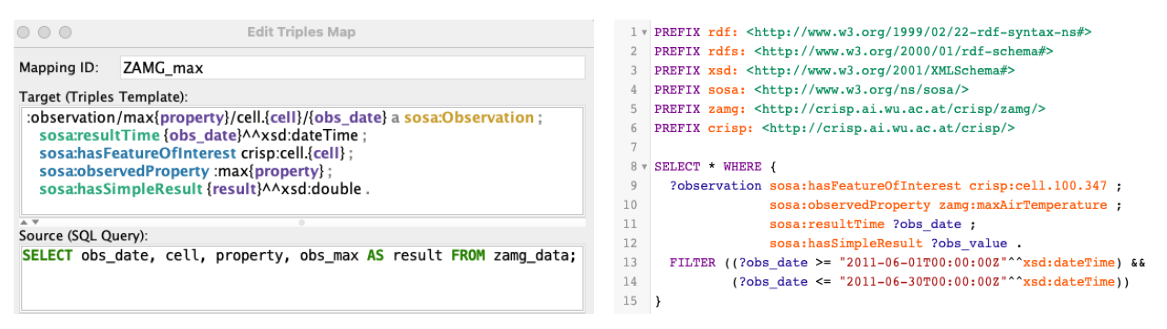
\includegraphics[width=\linewidth]{images/ZAMG_mapping.png}
  \caption{Weather data mapping and query.}
  \label{zamg_mapping}
\end{figure}


%%%%%%%%%%%%%%%%%%%%%%%%%%%%%%%%%%%%

\section{Conclusion and Future Work}

Complex interdependencies of infrastructure elements and service networks within the CRISP KG inform us about the potential impact of different types of shocks and stresses. They can help us develop more effective response strategies to mitigate the effects of future crises. We are currently enriching the CRISP KG based on the proposed modeling approach presented in this paper and address the technical challenges of big data integration. The next step towards achieving semantic interoperability in crisis management use cases is the integration of relevant crisis management processes and including access control in order to secure sensitive data and processes in the knowledge graph.




%%
%% The acknowledgments section is defined using the "acknowledgments" environment
%% (and NOT an unnumbered section). This ensures the proper
%% identification of the section in the article metadata, and the
%% consistent spelling of the heading.
\begin{acknowledgments}
% The authors acknowledge support from the Austrian Research Promotion Agency's ICT of the Future Program (FFG Project No. 887554.)
\end{acknowledgments}

%%
%% Define the bibliography file to be used
\bibliography{bibliography}

%%
%% If your work has an appendix, this is the place to put it.
\appendix


\end{document}

%%
%% End of file
